\section{Stage 3: Model Training} \label{sec:work_stage3_model_training}

Now, that all the energy profiles are collected it is possible to finally start training the models. As explained in \ref{sec:background_machine_learning} there are a lot of possible ways of using machine learning, however in this case the approach that best fit our need is supervised machine learning. So, some models were trained to see how good they performed using the data collected.

First there is a merge of features. While each method is initially trained individually, it is not useful to treat LinkedList.add(Object) and ArrayList.add(Object) as entirely separate cases. Both represent the same List.add(Object) method, differing only in their characteristics specific to their implementation. Therefore, once all energy profiles have been collected, a merging step is performed to consolidate these related methods.

All these features are stored in a new CSV and for the python program in a Data frame, to be processed.

This part was developed in python using some libraries specialized on machine learning, like scikit-learn (sklearn)~\cite{scikit-learn} which contains some models and functions to evaluate the models, and PySR~\cite{cranmeR²023interpretablemachinelearningscience} which was already explained in \ref{sec:background_machine_learning} an is also already implemented.

In this phase the models tested were: Decision Tree Regressor, Random Forest, Gradient Boosting, Linear Regression, and PySR.

\begin{figure}[htbp]
  \centering
  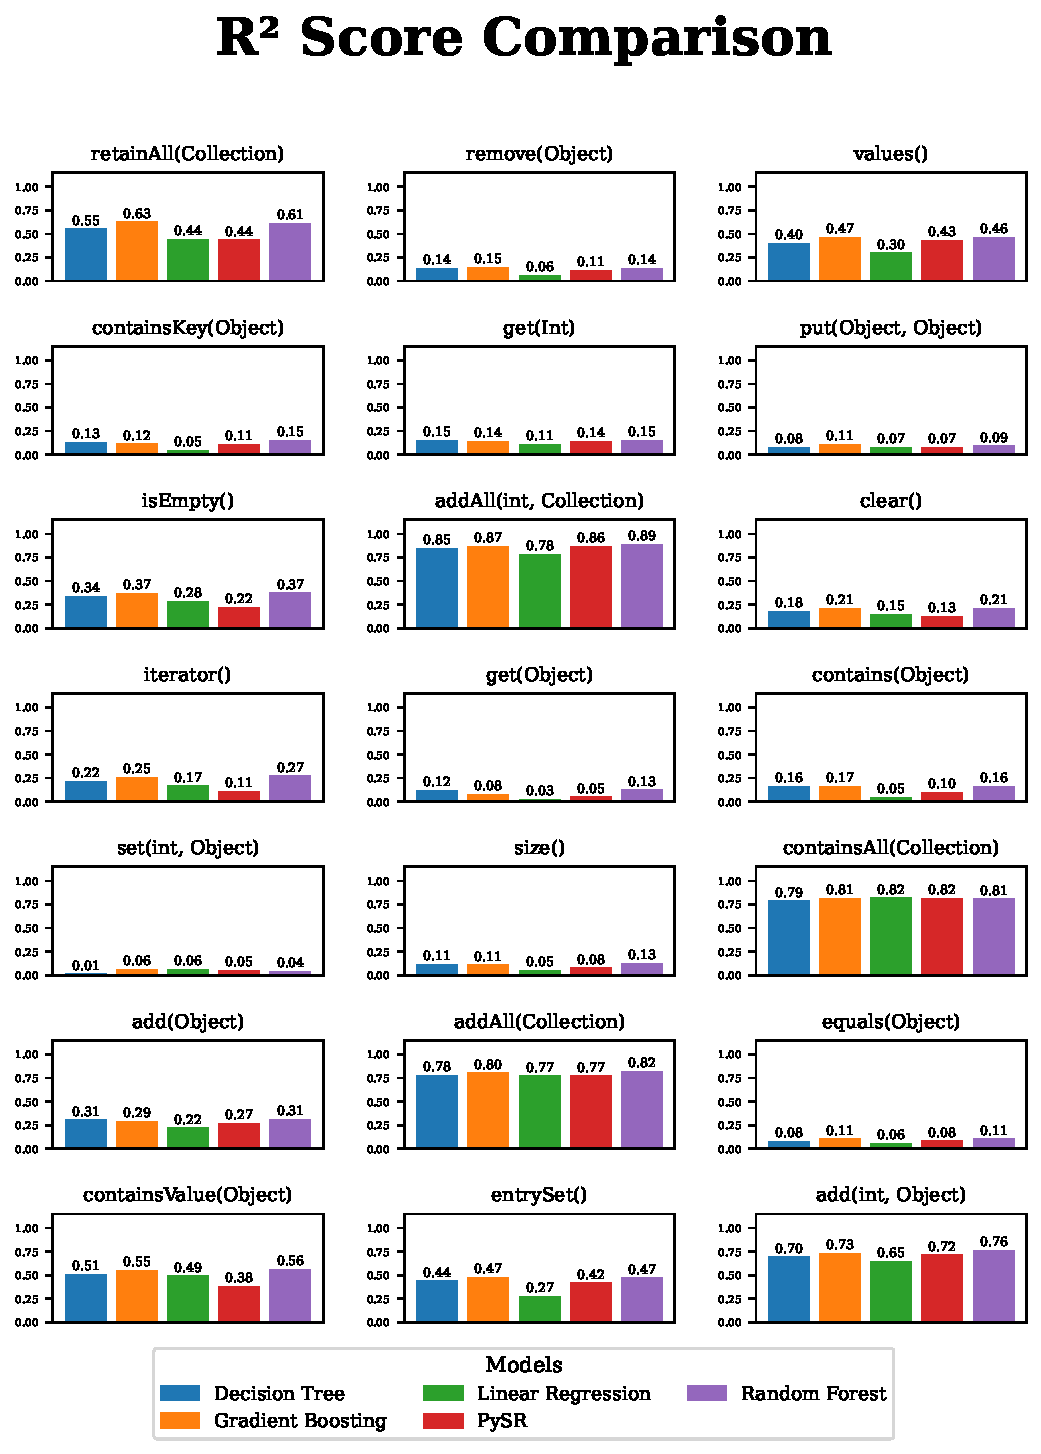
\includegraphics[width = .8 \textwidth]{figures/r2_comparison.pdf}
  \caption{R² Comparison}
  \label{fig:r2_comparison}
\end{figure}

\begin{figure}[htbp]
  \centering
  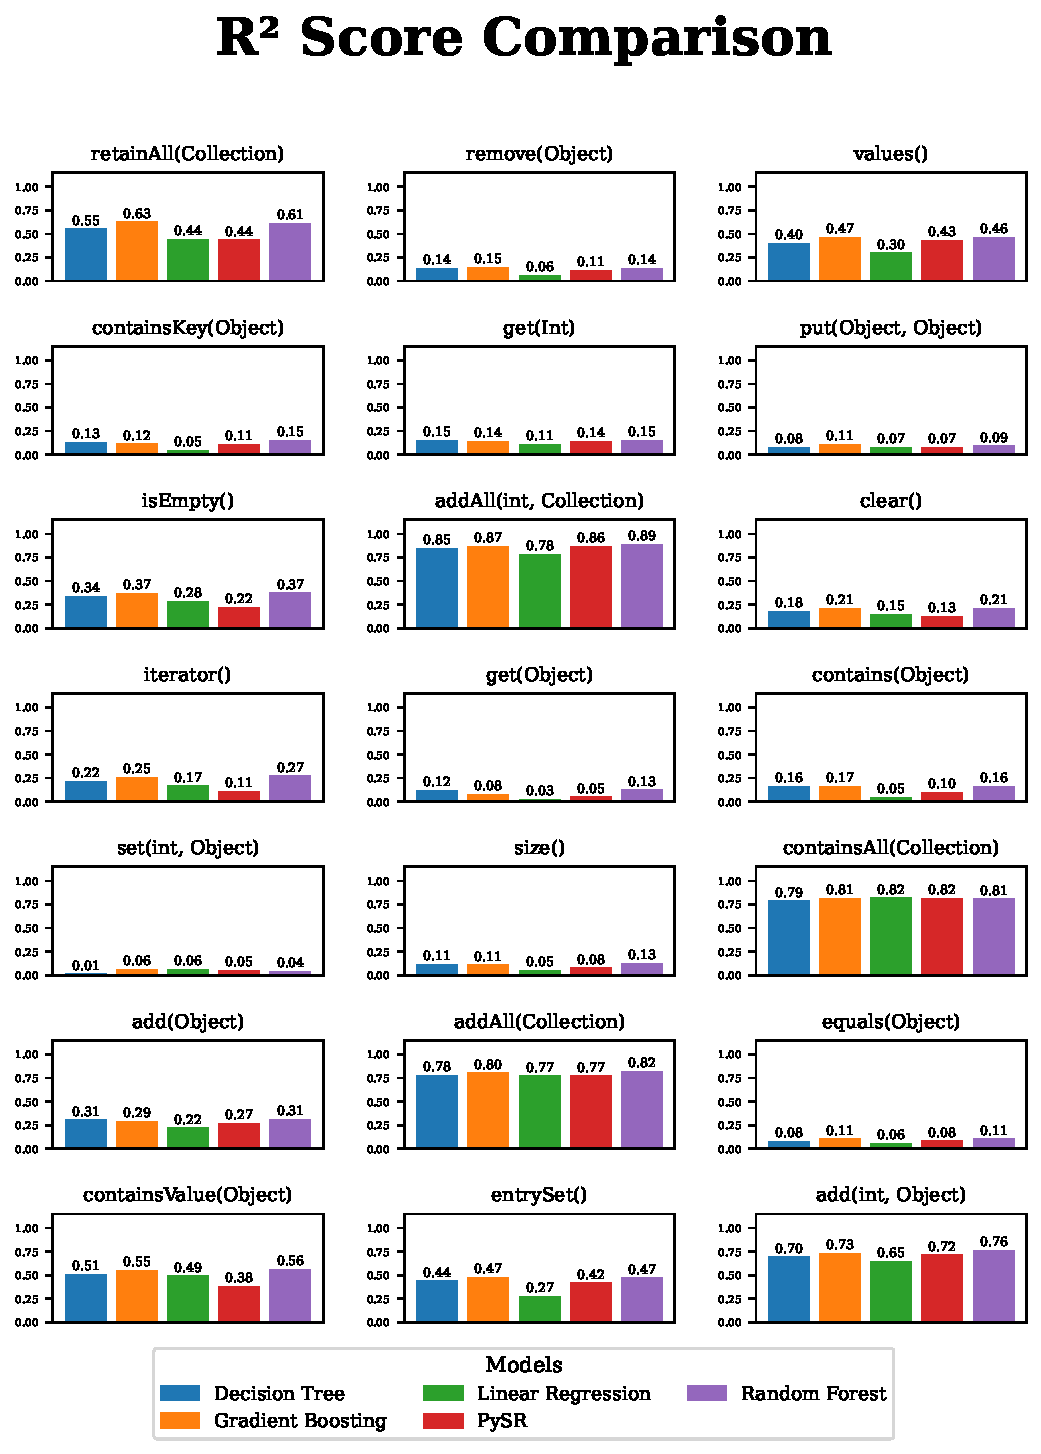
\includegraphics[width = .8 \textwidth]{figures/r2_comparison.pdf}
  \caption{MSE Comparison}
  \label{fig:mse_comparison}
\end{figure}

The results of the R² can be seen in the figure ~\ref{fig:r2_comparison}.
Ideally the best score is 1, meaning that the model can get 100\% of the prediction right, however that is not possible in most cases, and this project is not an exception to the rule. It is noticeable that most values are really low (bellow 0.8), which means that the model cannot predict the energy very well for some methods. The best models were for the method addAll and containsAll of the List collection, which got an R² of around .8 for most models, meaning that for those 3 methods on average the predictions will be 80\% correct.

For the other methods the scores were lower. The explanation found for this result was the following:


\begin{figure}[htbp]
  \centering
  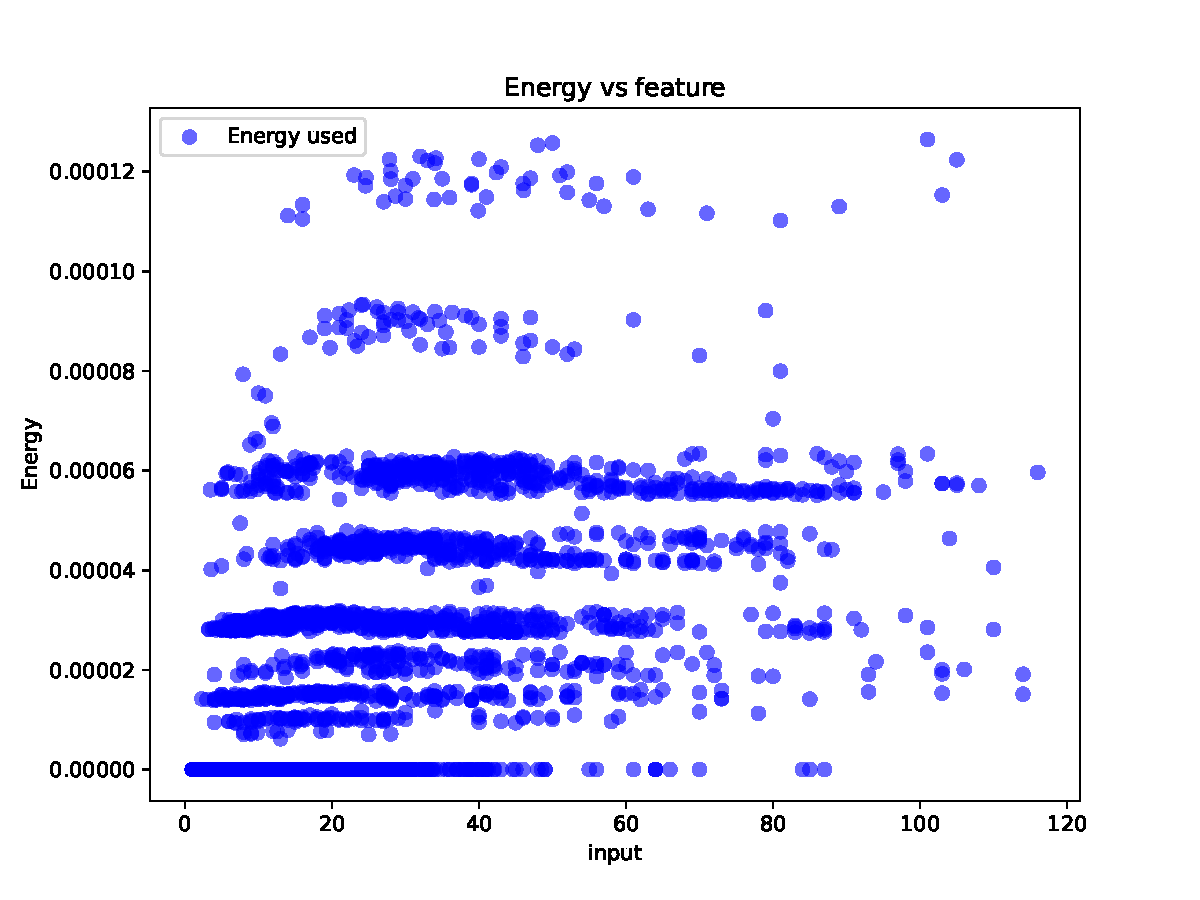
\includegraphics[width = .8 \textwidth]{figures/size_energy.pdf}
  \caption{Energy for the size method with different list sizes.}
  \label{fig:size_energy}
\end{figure}

The 3 methods with the most accuracy were the ones that generated bigger energy outputs, because the methods were computationally more powerful than the others. This made it so that bigger inputs would result in bigger energy outputs, and make the models more easily find a pattern to predict the energy. As for the other models, since a bigger input would not mean a bigger energy output, the model, might had some difficulties predicting the energy. This does not mean that a lower R² will completely make the model unusable for some methods, as their MSE, that can be seen in the figure ~\ref{fig:mse_comparison} is not high, meaning that even when failing to predict the energy of the method, the failed prediction will not be far away as one might expect. For example, if a model has an MSE of $1 \times 10^{-10}$ and predicts the energy usage to be $1~\mathrm{J}$, then even if the prediction is not exact, the true value is likely within $\pm \sqrt{1 \times 10^{-10}} = \pm 1 \times 10^{-5}~\mathrm{J}$ of the prediction, indicating accurate performance despite a potentially low R². 

Another factor that may contribute to low R² scores is the behavior of the energy measurement tool when applied to certain methods. For instance, some methods, such as \texttt{size()}, do not require more computational effort as the collection size increases. Whether the collection has one element or one million, the method executes in roughly the same amount of time. Consequently, the energy consumption remains nearly constant, regardless of the input size. Since these methods complete very quickly and consume very little energy, even minimal measurement noise can significantly affect the recorded values. Figure~\ref{fig:size_energy} illustrates this effect: although an increase in energy with input size is typically expected, the recorded energy values for \texttt{size()} remain considerably flat. While this example isolates a single feature, and other features also influence energy consumption, input size is often the most significant. This observation suggests that for low-energy, low-variance methods, measurement noise can impact the signal, making accurate energy prediction particularly challenging.


Nonetheless, the lower R² scores should be addressed, and what can be done to improve the results of these models is to have the program generator create higher inputs, so the energy profiles also have outputs with higher energy, making the energy predictions more accurate. Then, since most of the predictions depend on the input, it means the other features do not have such higher impact, so it is also important to pick better features and remove others that might not be so interesting. 



First the values of the MSE and R² are evaluated by the default values of sklearn, then in a second pass, GridSearch was used, which is a function of sklearn that tries to find the best parameters for a model. After that the scores and models are saved. The GridSearch does not work with PySR as they are from different libraries so, the parameters for PySR were manually set.

In the end the chosen model was PySR as it can represent the predictions in expressions which can help the users to try to understand why the code is using more energy. It has a nice feature of allowing to balance complexity and accuracy. And can easily be used in another code language as it is represented as a mathematical expression.

